\chapter{Background \& Related Work}
\label{chp:background}

In this chapter, the background and related work is discussed. In Section~\ref{sec:background}, fundamental concepts are explained which are used in this thesis. In Section~\ref{sec:related_work} the building blocks are laid out, on which this project has been build.

\section{Background}
\label{sec:background}
% More explanation on the concepts behind the techniques used. Explanation on radar, the chips etc.
% To explain:
% - Heart rate detection methods
% - mmWave technology
% - chirps
% - FFTs
\subsection{mmWave technology}
The type of radar used in this project is the \emph{Texas Instruments IWR6843ISK}, see Figure~\ref{fig:iwr6843isk}. This is a FMCW (Frequency Modulated Continuous Wave) radar. It uses short-wavelength elektromagnetic waves with a frequency of typically between 60-81 GHz, which means that it is legal to use in the Netherlands~\cite{freq_plan}. The TI package that is used in this project is an all-in-one solution. It contains the Tx and Rx analog circuitry to generate and capture the RF signals. It also contains analog-to-digital converters (ADCs), microcontrollers (MCUs) and digital signal processors (DSPs) to make signal processing possible all on the chip. It also has some custom hardware accelerators build in to speed up standard radar calculations, such as the generation of an fast fourier transforms (FFTs).

\begin{figure}[t]
\centering
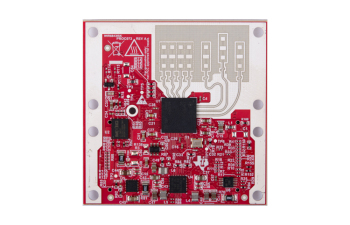
\includegraphics[width=.5\textwidth]{figures/iwr6843isk.jpg}
\caption{The Texas Instruments IWR6843ISK. This module is used throughout the project.}
\label{fig:iwr6843isk}
\end{figure}

\subsubsection{Chirps}
The fundamental concept in radar systems is the transmission of an electromagnetic signal, which is reflected on a target and then received by the radar again. FMCW radars make use of a special kind of signal. The frequency of this signal increases linearly over time, this type of signal is also called a chirp. See Figure~\ref{fig:chirp} for an example chirp waveform, with on the y-axis the magnitude and on the x-axis time. Chirps can be defined by three parameters: frequency ($f_c$), bandwidth ($B$) and duration ($T_c$). A chirp has also a slope ($S$), which captures the rate of change of frequency. There are a lot of parameters which can be set to modify the chirp. In this way the chirp can be tuned to provide information which is important for the application. The main balance which needs to be found is range versus resolution. The signals from the sensor can reach up to 150 meters away, but the resolution will drop to around 4 centimeters. When the sensor is setup to have a range of 2 meters, the resolution can be as low as a couple of millimeters.

\begin{figure}[t]
\centering
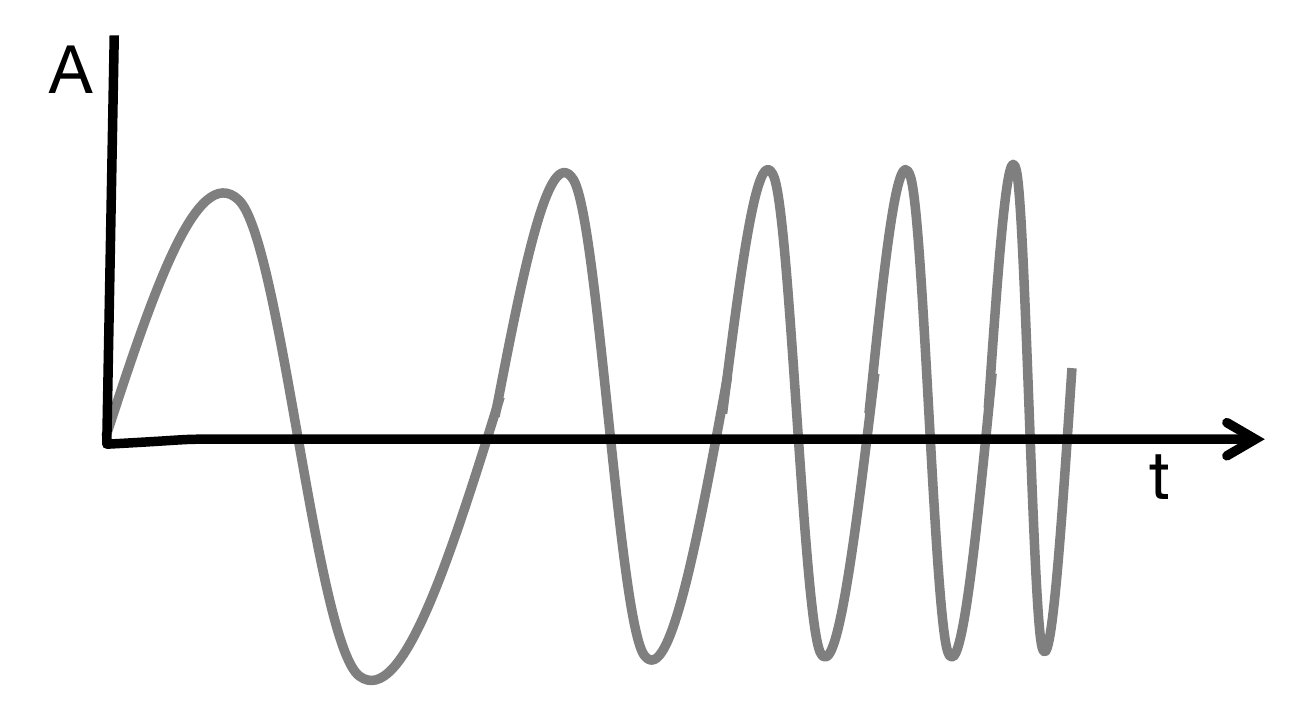
\includegraphics[width=.5\textwidth]{figures/chirp.png}
\caption{Chirp signal, with the amplitude as a function over time.}
\label{fig:chirp}
\end{figure}

\subsection{Range estimation}
In Figure~\ref{fig:fmcw_inner}, a scheme of the inner workings of the FMCW chip can be found. First, a chirp is generated using the synth (1). This chirp is then transmitted over one or multiple Tx antenna (2). When reflected on an object, the signal returns and is captured using the Rx antenna (3). During the travel of the signal, the frequency changes. The further the object is away from the sensor, the more the frequency changes. The signal from the synth and the received signal from the Rx antenna get mixed (4). This mixer has two signals as input, and one signal as an output. The mixer outputs a signal with a frequency which is the difference between the two input frequencies. This output signal is called the intermediate frequency (IF) signal. In Figure~\ref{fig:if_signal} the situation is displayed more visually. Using this information we can use the equation

\begin{equation}
\tau = \frac{2d}{c}
\label{eq:range_equation}
\end{equation}

where $\tau$ is the time delay and $c$ is the speed of light, to compute the distance to the object $d$. 

This is an example where only one object is used. But in the real world, there are almost always more objects to be detected. All of these objects return another reflection, which means that one transmitted signal from the Tx antenna can result in multiple reflections reaching the Rx antenna, as depicted in Figure~\ref{fig:if_multiple}. In this instance, there are multiple IF tones at once, one for each reflected object. To differentiate between those, we make use of a Fourier transform. After processing this Fourier transform, it results in a frequency spectrum in which each peak will point to one separate IF frequency. The IWR6843 has a hardware accelerator to speed up the Fourier transform generation.

% TODO: calculations for distance in meters using FFT?

\begin{figure}[t]
\centering
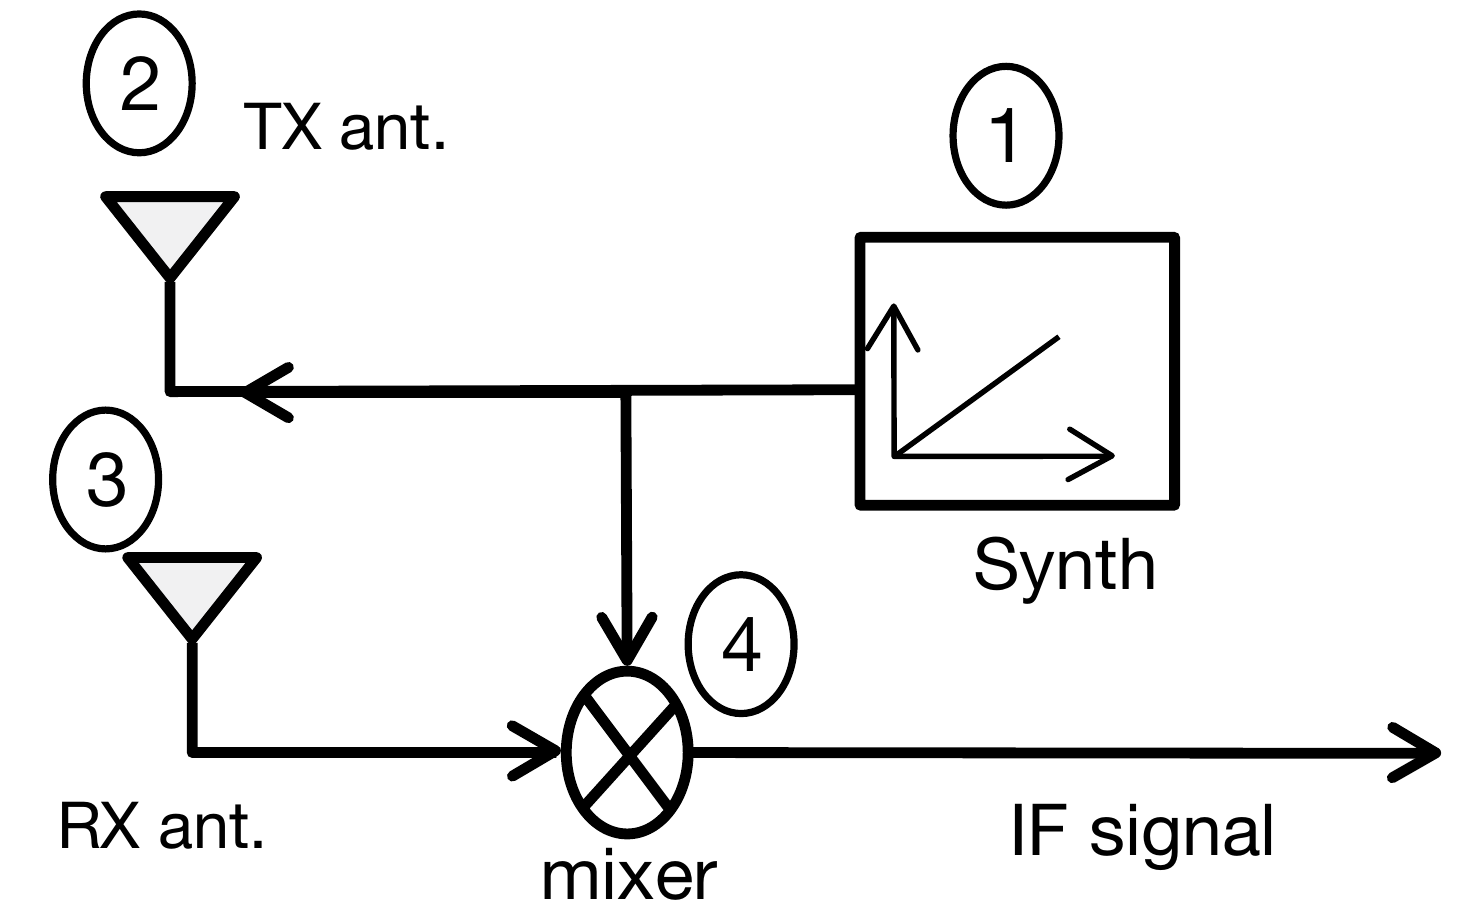
\includegraphics[width=.5\textwidth]{figures/fmcw_internals.png}
\caption{Scheme of the inner workings of the FMCW chip.}
\label{fig:fmcw_inner}
\end{figure}

\begin{figure}[t]
\centering
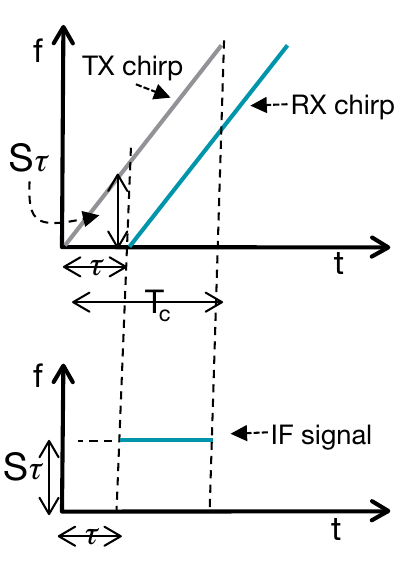
\includegraphics[width=.5\textwidth]{figures/if_signal.png}
\caption{The calculation of the IF signal. In the top graph, the Tx and Rx chirp are plotted. In the bottom graph, the IF signal is plotted.}
\label{fig:if_signal}
\end{figure}

\begin{figure}[t]
\centering
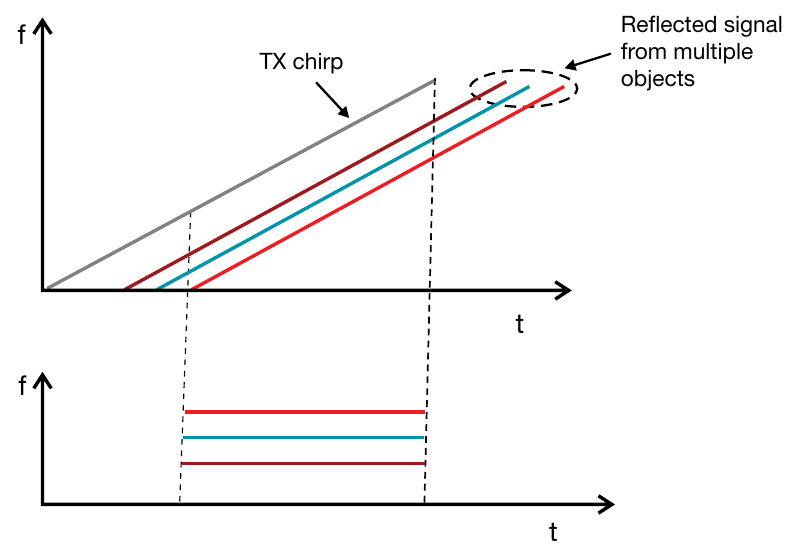
\includegraphics[width=.5\textwidth]{figures/reflected_signals.png}
\caption{One Tx signal can result in multiple reflections on the Rx antennas from multiple objects in front of the sensor.}
\label{fig:if_multiple}
\end{figure}

\subsection{Doppler estimation}
The range information, calculated using the range-FFT, is also known as the 1D-FFT. Most of the time, this is the first processing step for radar data. But, there is more information we can extract from the radar data. Sometimes it is useful to know the velocity of objects. 

To calculate the velocity of objects, we need the data from the range-FFT. The radar transmits two chirps, spaced $T_c$ apart from each other. Both of these chirps get reflected on the object and for both of them a range-FFT is calculated. Because the chirps are transmitted almost immediately after each other, the two FFTs have peaks in the exact same location. What matters now is the phase of the peaks. The output of a FFT is an array of complex numbers. The real part says something about the frequency of the signal, the imaginary part says something about the phase of the sinusoidal signal. The phase between the two chirps is changed slightly because even between those two chirps spaced $T_c$ apart, the object moved. The velocity can be derived using this formula:

\begin{equation}
v = \frac{\lambda \Delta \phi}{4 \pi T_c}
\label{eq:doppler_equation}
\end{equation}

Because the velocity is dependent on the phase value, the velocity could wrap around if the object is moving too fast. Therefore, the maximum speed the radar is able to record before the measurements start to be untrustworthy, is:

\begin{equation}
v_{max} = \frac{\lambda}{4 T_c}
\label{eq:doppler_equation_max_speed}
\end{equation}

To determine the velocities of multiple objects, a FFT is used to differentiate between multiple objects. In the example above for only one object, two chirps are needed to calculate the velocity of the object. To distinguish between multiple objects, more chirps are needed. Each chirp is one input data element for the FFT, so the more chirps, the more accurate the result. All of those chirps together forming the data for the range-FFT and the doppler-FFT are called a frame. 

\subsection{Angle estimation}
Using the methods above, we can estimate the range and the velocity of multiple objects using range- and doppler-FFTs. But, there is still one more shortcoming of these calculations. They only work for one dimension. This means that if object 1 is 3 meters from the sensor and object 2 is 5 meters from the sensor, everything is fine. But, if two objects are at the same distance to the sensor but with a different angle, these two objects would get merged into one. The solution to this problem is to try and calculate the angle of the object with respect to the sensor, also known as the Angle of Arrival (AoA). This way, the data collection from the sensor can be expanded from one dimension into two dimensions.

To calculate the Angle of Arrival, multiple Rx antennas are needed. In Figure~\ref{fig:angle_estimation} the functional diagram of how angle estimation works is displayed. A chirp is emitted from a Tx antenna. The chirp is reflected on an object and received by the first Rx antenna. The distance between the object and the Rx antenna is $d$. When the signal arrives at the second Rx antenna, it has traveled $d + \Delta d$. Because of this $\Delta d$, the phase on the second Rx antenna is different from the first Rx antenna. A similar formula as the doppler estimation can be formed to tie these concepts together:

\begin{equation}
\Delta \phi = \frac{2 \pi \Delta d}{\lambda}
\label{eq:angle_equation}
\end{equation}

Using some basic geometry, we can deduce the formula for the angle of arrival using Eq. \ref{eq:angle_equation}:

\begin{equation}
\theta = \arcsin{\frac{\lambda \Delta \phi}{2 \pi l}}
\label{eq:angle_equation_2}
\end{equation}

Using multiple Rx antennas, in the case of this project using the IWR6843ISK there are 4 antennas, we can calculate the AoA of different objects using a FFT. At this point, a 2D heatmap can be constructed using the calculations from the different estimations above. This heatmap is the starting point for this project.

\begin{figure}[t]
\centering
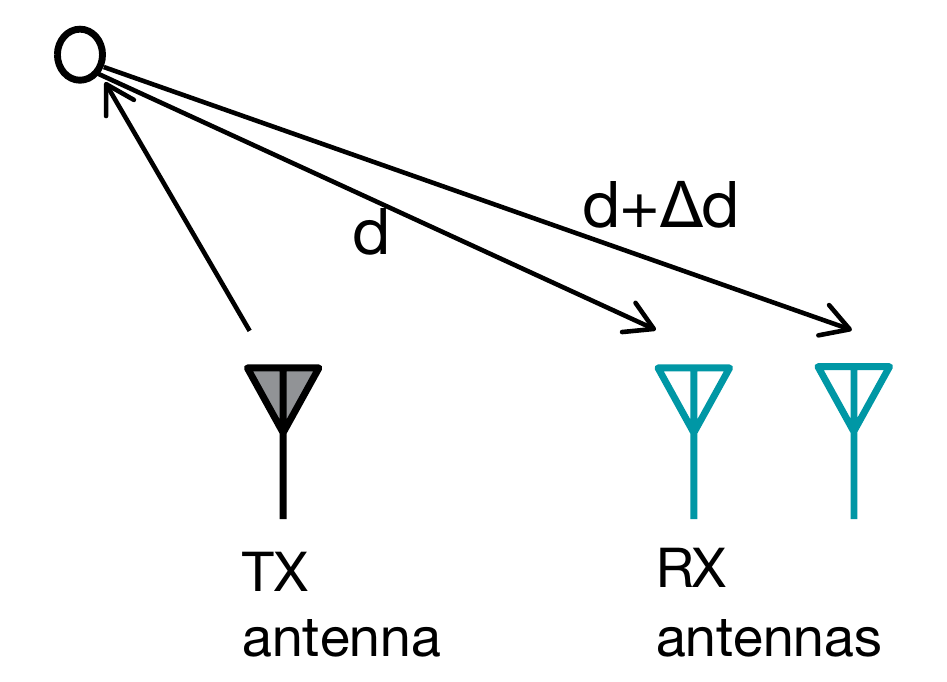
\includegraphics[width=.5\textwidth]{figures/angle_estimation.png}
\caption{One Tx signal is received by multiple Rx antennas. Because the signal travels $\Delta d$ longer to one Rx antenna compared to the other, the angle of arrival can be calculated.}
\label{fig:angle_estimation}
\end{figure}

\section{Related Work}
\label{sec:related_work}
% Use building blocks for the related work. What is new? So start with app1, app2 and app3, and based on these you end up with app4. With app4 you define something novel for example. So, describe this path
% Papers to use:
% - Monitoring Vital Signs Using Millimeter Wave \cite{yang2016monitoring}
% - Vital signs monitoring of multiple people using a FMCW millimeter-wave sensor \cite{ahmad2018vital}
% - Radar remote monitoring of vital signs \cite{li2009radar}
Using radar to estimate vital signs has already been researched before. One of the first papers about the subject is \cite{li2009radar}, which uses a transmitter to send a unmodulated signal to a patient and receive the modulated signal back. The signal gets demodulated and the heart rate and breathing rate can be extracted. In this attempt, a lot of analog hardware is used to make the vital signs extraction work. 

A similar attempt has been made by \cite{yang2016monitoring}. The researchers made use of two separate antennas, one for transmitting and one for receiving. The transmitting antenna does a first sweep through the room by physically moving the antenna to detect persons in the room. After that, the transmitter and receiver can zone in on the person and detect the vital signs of that person. The transmitting and receiving is done with large pieces of equipment. 

In \cite{alizadeh2019remote} the step to FMCW radars can be observed. The authors also use a chip from TI, but an earlier model. They make use of a range-FFT to detect a person, and perform vital signs estimation on that person. A disadvantage of this approach is that the solution is only able to estimate the vital signs of one person. Another disadvantage is that the data gathered by the sensor is send to a computer for processing at a later time. This means that the vital signs estimation is not real time. 

The paper which is closest to the research topic of this paper, is \cite{ahmad2018vital}. The authors from this paper all work for TI, and made a proof of concept solution for multiple person vital signs estimation using a TI sensor. The sensor first looks for persons in the 2D space before the sensor. Then, it uses a special kind of beamforming technique to isolate the data for one person at a time to extract the vital signs. It does this for all of the persons within reach of the sensor. Again, there are some disadvantages with this method. Firstly, the special beamforming technique they are using to isolate the different persons from each other is not shown in detail. When asked if they could share their code, it appeared to be under an NDA. The most important disadvantage is that the calculations are done in Matlab after the data gathering. In the medical world, it is important to have information about a patient right away, and not minutes to hours after they have been recorded. 